\RequirePackage{pdf14}
\documentclass[aspectratio=169]{beamer}
\mode<presentation>

\hypersetup{pdfpagemode=FullScreen}
\useoutertheme[subsection=false]{smoothbars}

\usepackage[utf8]{inputenc}
\usepackage{tikz}
\usetikzlibrary{shapes}
\usetikzlibrary{arrows.meta}
\usepackage{listings}
\graphicspath{{res/}}

\colorlet{punct}{red!60!black}
\definecolor{delim}{RGB}{20,105,176}

\lstdefinelanguage{json}{%
	basicstyle=\scriptsize\ttfamily,
	showstringspaces=false,
	breaklines=true,
	literate=
		*{:}{{{\color{punct}{:}}}}{1}
		{,}{{{\color{punct}{,}}}}{1}
		{\{}{{{\color{delim}{\{}}}}{1}
		{\}}{{{\color{delim}{\}}}}}{1}
		{[}{{{\color{delim}{[}}}}{1}
		{]}{{{\color{delim}{]}}}}{1}
}

\lstdefinelanguage{dockerfile}{%
	basicstyle=\ttfamily,
	showstringspaces=false,
	breaklines=true
}
\lstset{language=dockerfile}

\lstdefinelanguage{caveats}{%
	basicstyle=\scriptsize\ttfamily,
	showstringspaces=false,
	breaklines=true
}

\tikzset{%
	arrow/.style={%
		draw,
		fill=structure.fg,
		single arrow,
		minimum width=5ex,
		minimum height=10ex,
		single arrow head extend=1ex
	}
}
\newcommand{\arrow}{%
\tikz [baseline=-0.5ex]{\node [arrow] {};}
}

\title{\Huge Summary of Research Activities}
\subtitle{\LARGE Cycle XXXI (31)}
\author{\Large Yousef Amar\\\normalsize QMUL Supervisor: Hamed Haddadi\\\normalsize UNIGE Supervisor: Fabio Lavagetto}
\institute{\hspace{0.3cm}
\includegraphics[height=1.8cm]{qmul-logo}\hspace{1.3cm}
\includegraphics[height=1.8cm]{unige-logo}\hspace{0.9cm}
\includegraphics[height=0.8cm]{databox-logo}}
\date{2017-10-12}
\setbeamertemplate{navigation symbols}{}

\begin{document}

\frame{\titlepage}

\begin{frame}
	\frametitle{Research Context}
	\framesubtitle{The Databox Platform}
	\centering
	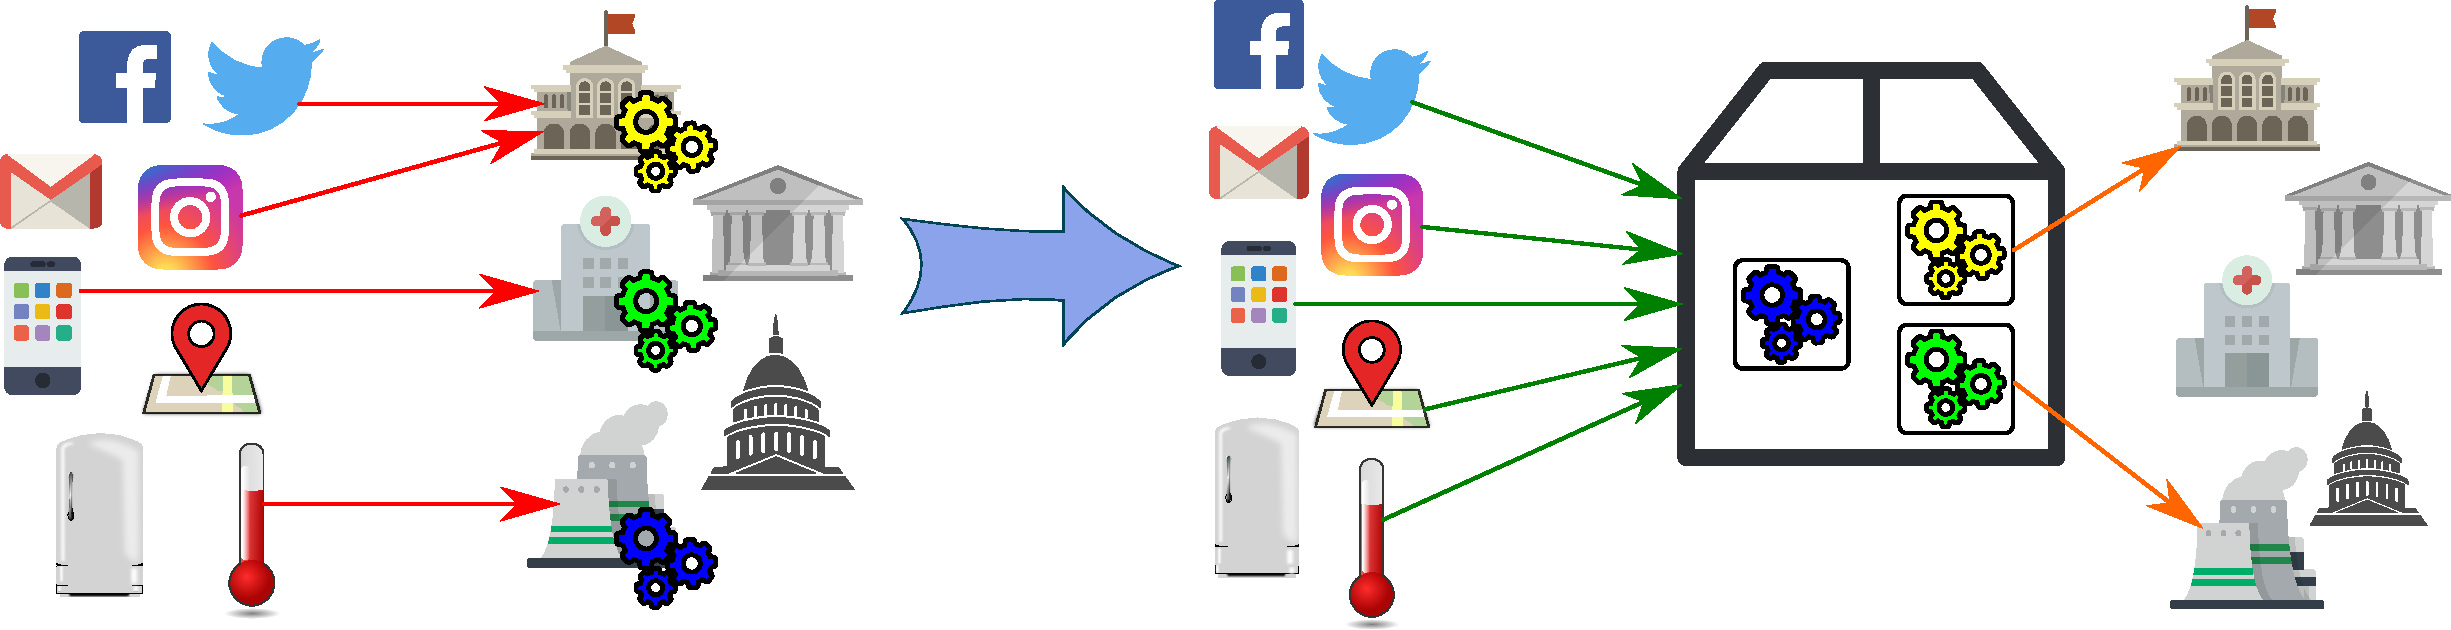
\includegraphics[width=\linewidth]{background}\\
\end{frame}

\begin{frame}
	\frametitle{Research Context}
	\framesubtitle{The Databox Platform}
	\centering
	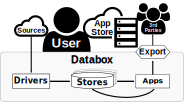
\includegraphics[width=0.7\linewidth]{databox-high}\\[1em]
	\pause
	\textit{How can we design safe, scalable access control systems\\with arbitrary restrictions in this context?}
\end{frame}

\begin{frame}
	\frametitle{Implementation}
	\centering
	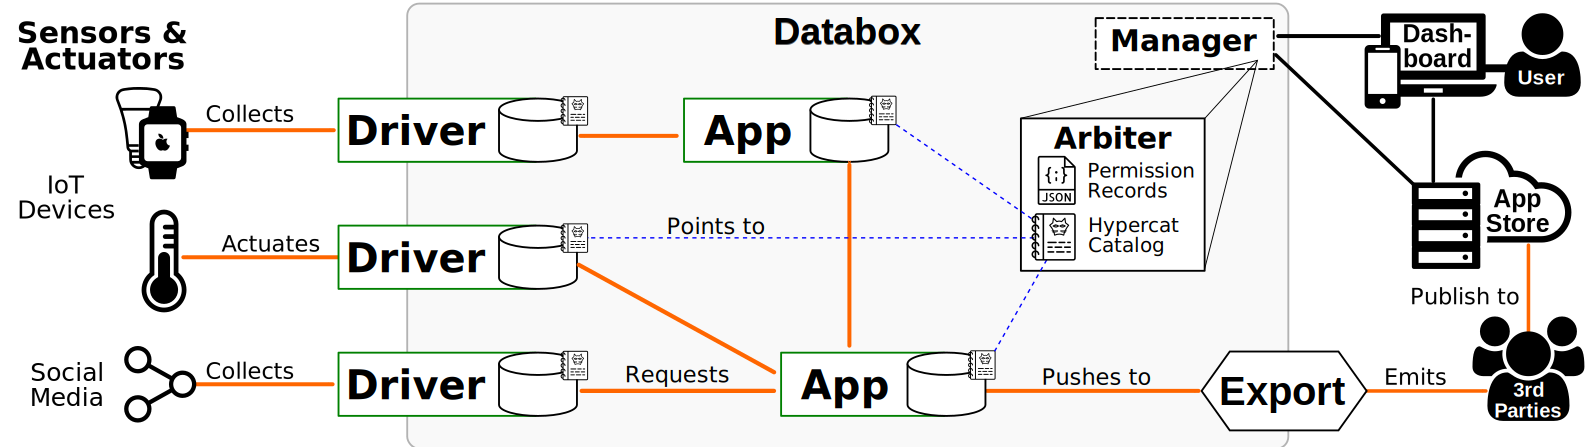
\includegraphics[width=\linewidth]{arch}\\
\end{frame}

\begin{frame}
	\frametitle{Evaluation}
	\begin{itemize}
		\item Scalability
		\begin{itemize}
			\item Resource usage (CPU, memory, network I/O)
			\item Inserts/s over stores under maximum load
			\item Store launch time with and without arbiter interaction (memory bottleneck)
		\end{itemize}
		\item Topology
		\begin{itemize}
			\item Device $\rightarrow$ Cloud
			\item Device $\rightarrow$ Cloud $\rightarrow$ Home
			\item Device $\rightarrow$ Home
			\item Device $\rightarrow$ Home $\rightarrow$ Cloud
		\end{itemize}
		\item Time to Availability -- High-frequency mobile sensors
	\end{itemize}
	\centering
	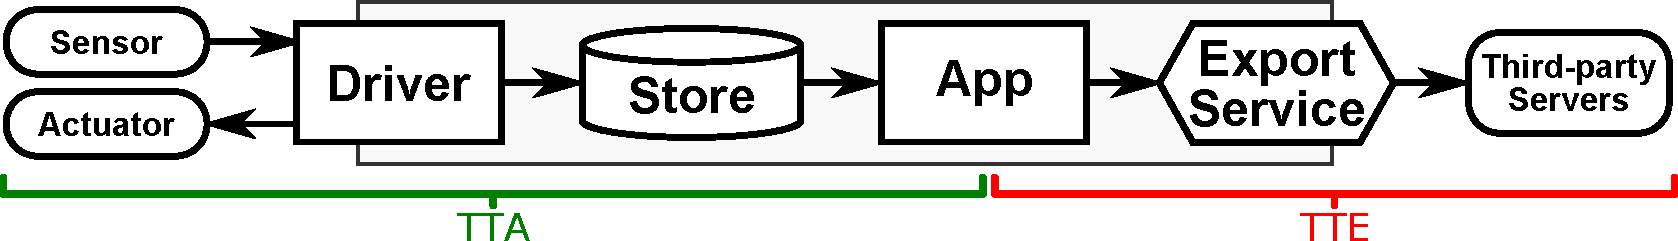
\includegraphics[width=0.8\linewidth]{tta-tte.pdf}
\end{frame}

\begin{frame}
	\frametitle{Research Context}
	\framesubtitle{The Serverless Paradigm}

	\begin{figure}
		\centering
		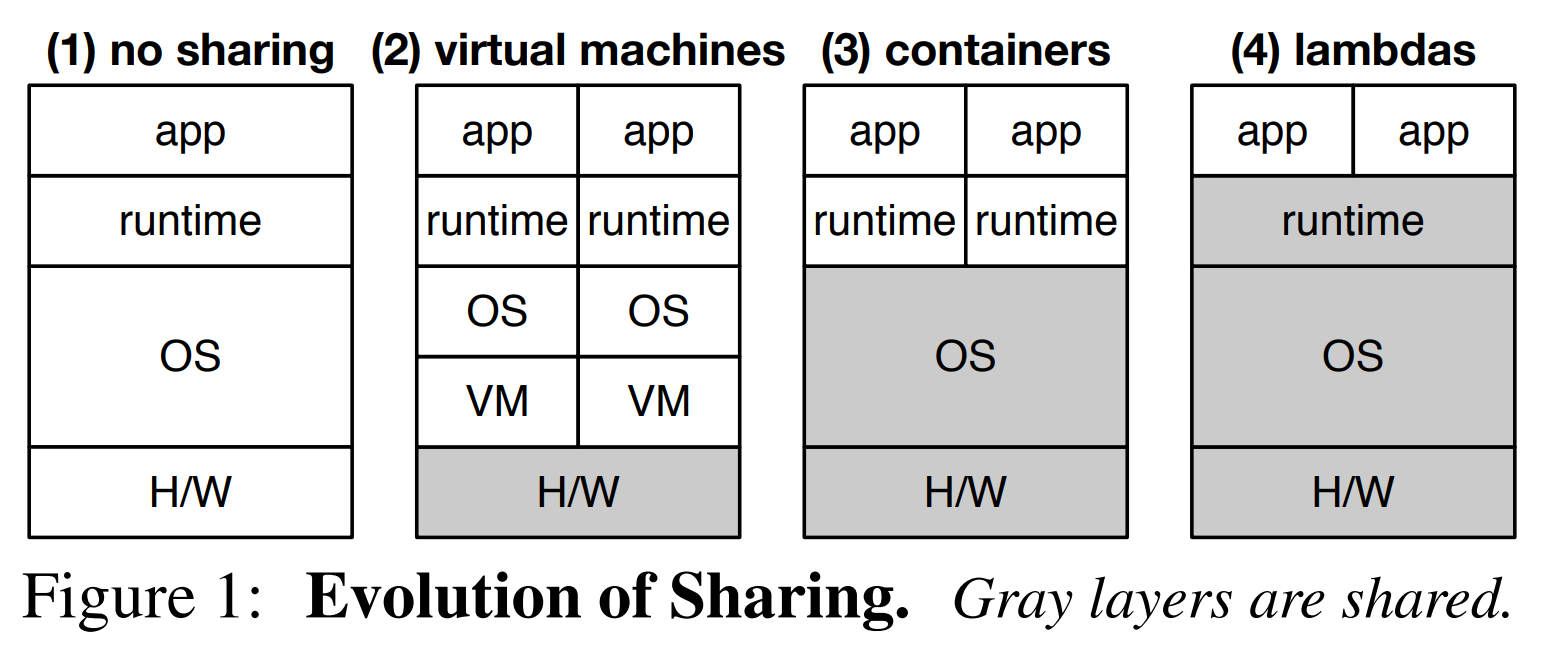
\includegraphics[width=\linewidth]{openlambda}
		\caption{Hendrickson, et al. ``Serverless computation with openlambda.'' Elastic 60 (2016): 80.}
	\end{figure}
\end{frame}

\begin{frame}
	\frametitle{Implementation}
	\framesubtitle{Low-latency Serverless}

	\begin{figure}[h]
		\centering
		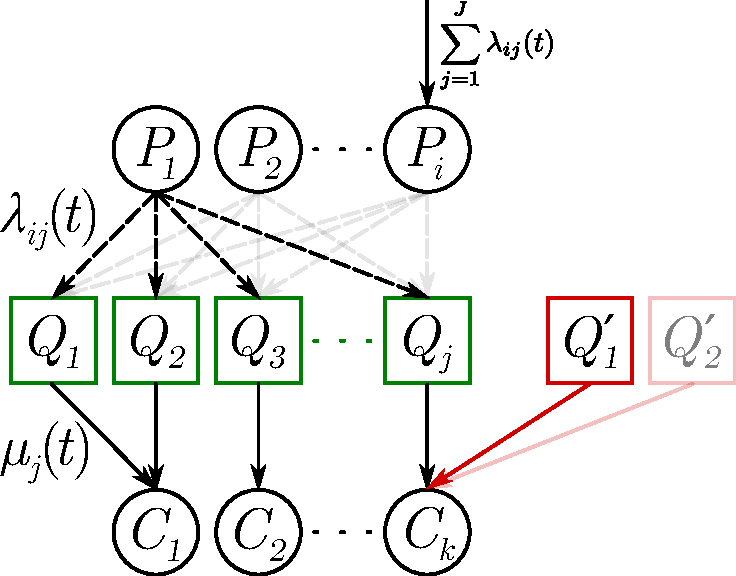
\includegraphics[width=0.5\textwidth]{diagram}
		\caption{An Overview of Inter-component Relationships}
	\end{figure}
\end{frame}

\begin{frame}
	\frametitle{Implementation}
	\framesubtitle{Low-latency Serverless}

	\begin{figure}[h]
		\centering
		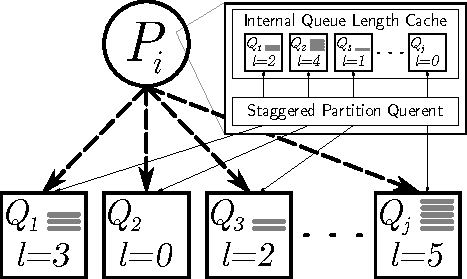
\includegraphics[width=0.7\textwidth]{cache}
		\caption{The Internal Components of a Producer}
	\end{figure}
\end{frame}

\begin{frame}
	\frametitle{Implementation}
	\framesubtitle{Low-latency Serverless}

	\begin{figure}[h]
		\centering
		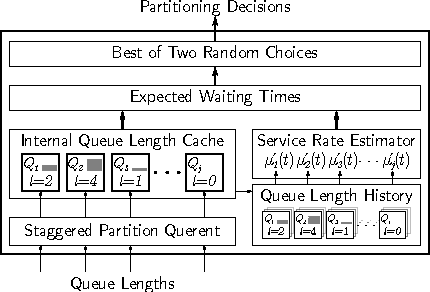
\includegraphics[width=0.6\textwidth]{service}
		\caption{Producer-intrinsic Steps for Computing Partitioning Decisions from Stale Queue Lengths}
	\end{figure}
\end{frame}

\begin{frame}
	\frametitle{Plans}
	\framesubtitle{Privacy and Risk Metrics}

	\begin{itemize}
		\item Measuring privacy risk is very subjective
		\item Information-theoretic, content-independent metrics are generalisable
		\item Looking just at metadata and schema of personal data, calculate objective metrics:
		\begin{itemize}
			\item k-anonymity
			\item l-diversity
			\item t-closeness
		\end{itemize}
		\item Thresholds can be embedded into tokens -- privacy-aware access control for free (!)
	\end{itemize}
\end{frame}

\begin{frame}
	\frametitle{Plans}
	\framesubtitle{Privacy and Risk Metrics}

	\begin{figure}[h]
		\centering
		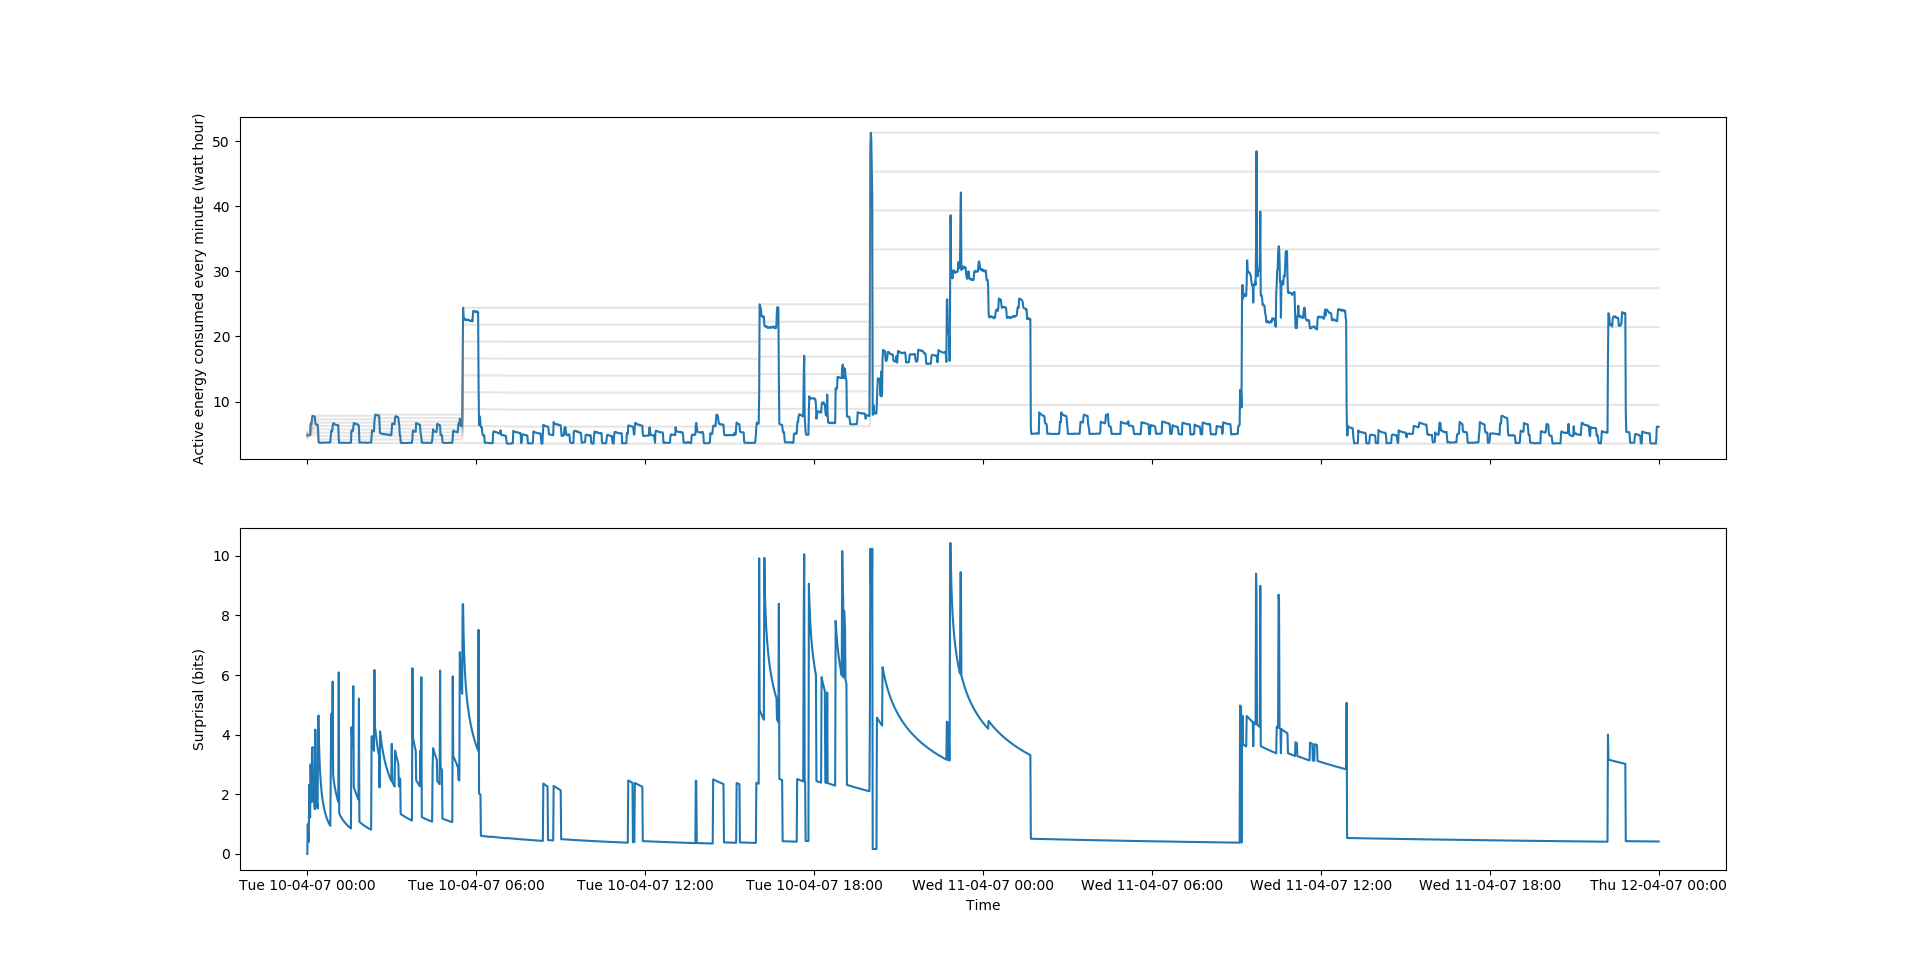
\includegraphics[width=0.8\textwidth]{surprisal}
		\caption{One Proof of Concept Experiment -- Surprisal over Real Smart Meter Data}
	\end{figure}
\end{frame}

\begin{frame}
	\frametitle{Plans}
	\framesubtitle{Serverless over Transient Clouds}

	\begin{columns}[c]
		\column{.5\textwidth}
		\begin{itemize}
			\item Serverless on the edge
			\item Optimising for context through latency
			\item Processor selection based on arbitrary metrics, e.g.\ surprisal
		\end{itemize}
		\column{.5\textwidth}
		\begin{figure}
			\centering
			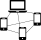
\includegraphics[width=0.8\columnwidth]{tcac}
		\end{figure}
	\end{columns}
\end{frame}

\begin{frame}
	\frametitle{Plans}
	\framesubtitle{Transient Privacy-Aware Clouds}

	\begin{columns}[c]
		\column{.5\textwidth}
		\begin{itemize}
			\item Encoding user-defined thresholds into bearer tokens
			\item Joint context at hierarchical levels
			\item TCACs $\to$ TPACs?
			%\item Arbiter token minting under load evaluation
			%\item Performance vs security when modifying token expiry
		\end{itemize}
		\column{.5\textwidth}
		\begin{figure}
			\centering
			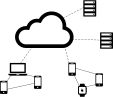
\includegraphics[width=\columnwidth]{tcacs}
		\end{figure}
	\end{columns}
\end{frame}

\begin{frame}
	\frametitle{The Big Picture}

	\begin{figure}[h]
		\centering
		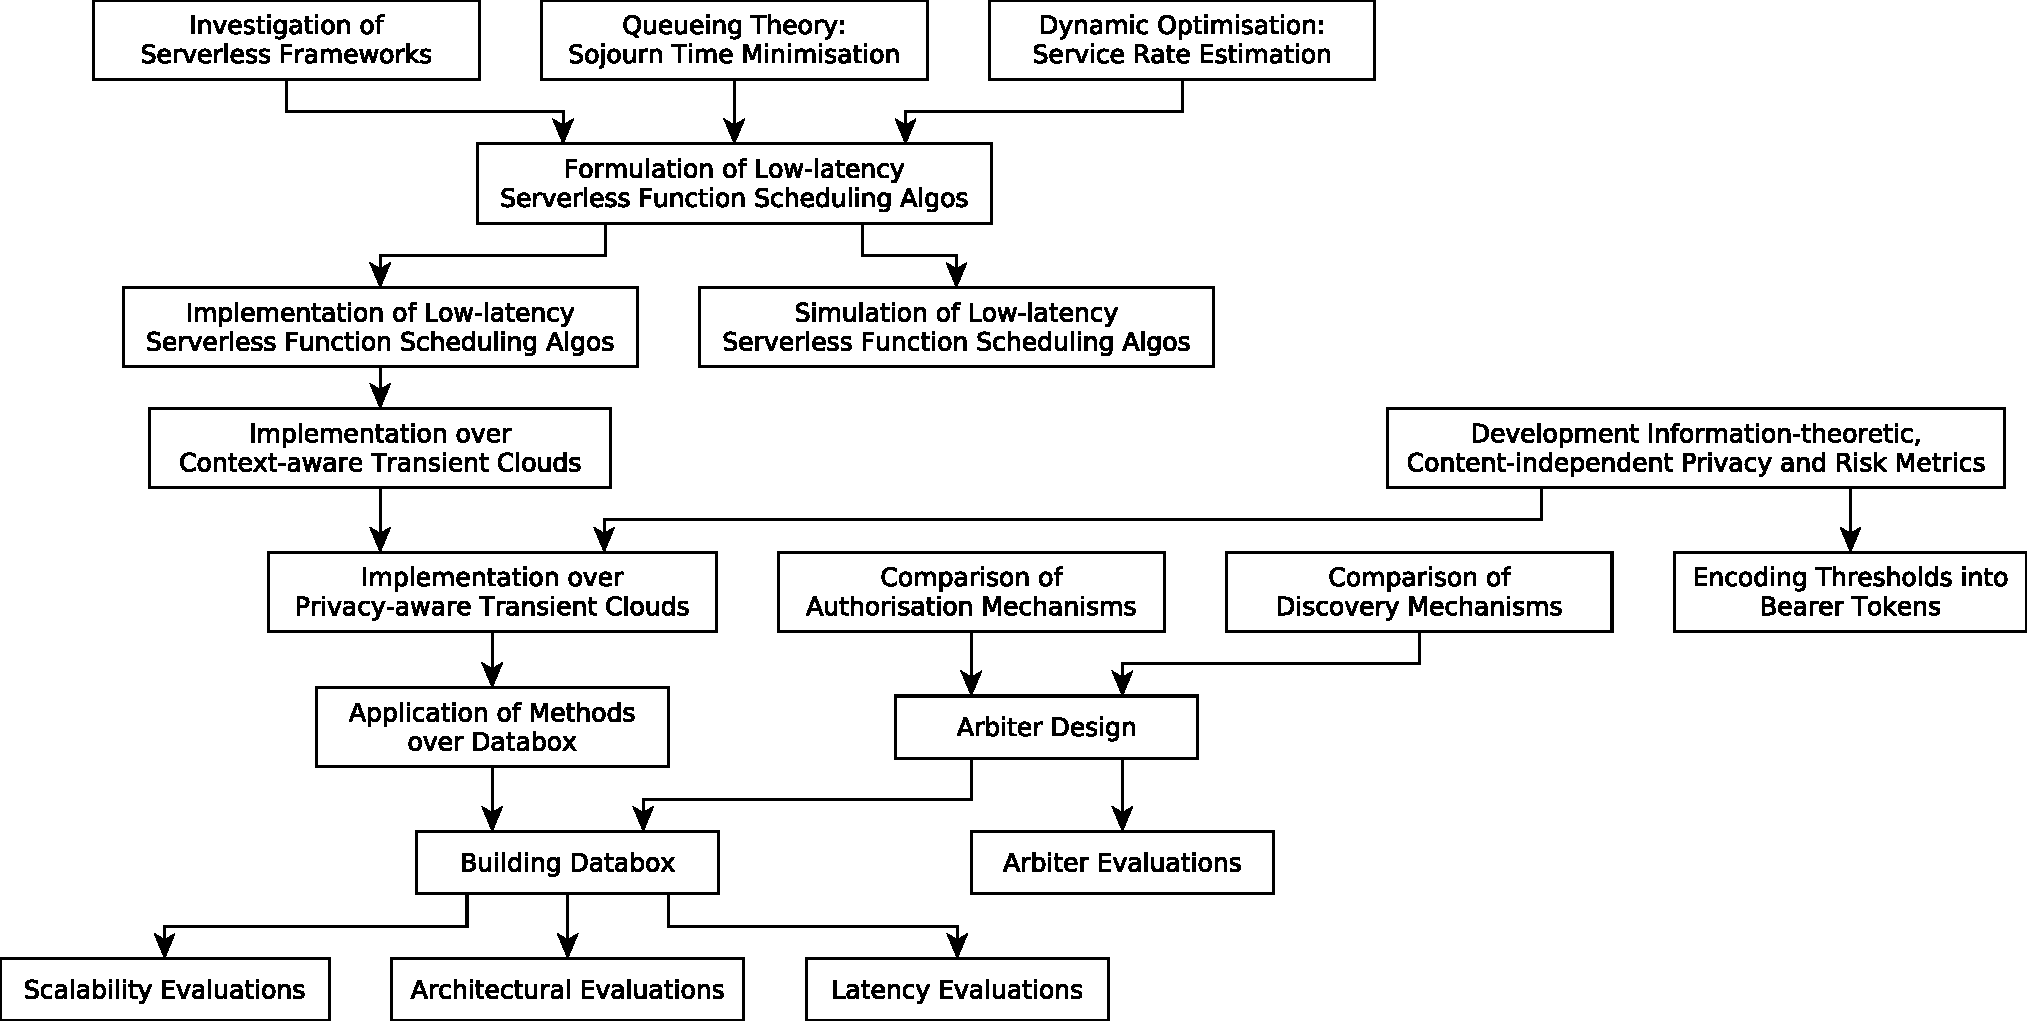
\includegraphics[width=0.8\textwidth]{dependencies}
		\caption{A High-level Dependency Graph of Research Activities}
	\end{figure}
\end{frame}

\begin{frame}[plain,c]
	\begin{center}
		\usebeamerfont*{frametitle}
		\usebeamercolor[fg]{frametitle}
		\\[4em]
		\Huge Thank you for your attention!\\[1em]
		\Large Questions?\\[1em]
	\end{center}
	\footnotesize
	\begin{table}[]
		\begin{tabular}{ll}
			More info:&\texttt{http://yousefamar.com/}\\
			Slides at:&\texttt{https://github.com/yousefamar/unige-presentation-year2}
		\end{tabular}
	\end{table}
\end{frame}

\end{document}
